% --------------------------------------------------------------
% This is all preamble stuff that you don't have to worry about.
% Head down to where it says "Start here"
% --------------------------------------------------------------

\documentclass[12pt]{article}

\usepackage[margin=1in]{geometry}
\usepackage{amsmath,amsthm,amssymb}
\usepackage{graphicx} %This allows to include eps figures
\usepackage{subcaption}
\usepackage[section]{placeins}
\usepackage{layout}
\usepackage{etoolbox}
\usepackage{mathabx}
% This is to include code
\usepackage{listings}
\usepackage{xcolor}
\definecolor{dkgreen}{rgb}{0,0.6,0}
\definecolor{gray}{rgb}{0.5,0.5,0.5}
\definecolor{mauve}{rgb}{0.58,0,0.82}
\lstdefinestyle{Python}{
    language        = Python,
    basicstyle      = \ttfamily,
    keywordstyle    = \color{blue},
    keywordstyle    = [2] \color{teal}, % just to check that it works
    stringstyle     = \color{green},
    commentstyle    = \color{red}\ttfamily
}

\newcommand{\N}{\mathbb{N}}
\newcommand{\Z}{\mathbb{Z}}

\newenvironment{theorem}[2][Theorem]{\begin{trivlist}
\item[\hskip \labelsep {\bfseries #1}\hskip \labelsep {\bfseries #2.}]}{\end{trivlist}}
\newenvironment{lemma}[2][Lemma]{\begin{trivlist}
\item[\hskip \labelsep {\bfseries #1}\hskip \labelsep {\bfseries #2.}]}{\end{trivlist}}
\newenvironment{exercise}[2][Exercise]{\begin{trivlist}
\item[\hskip \labelsep {\bfseries #1}\hskip \labelsep {\bfseries #2.}]}{\end{trivlist}}
\newenvironment{reflection}[2][Reflection]{\begin{trivlist}
\item[\hskip \labelsep {\bfseries #1}\hskip \labelsep {\bfseries #2.}]}{\end{trivlist}}
\newenvironment{proposition}[2][Proposition]{\begin{trivlist}
\item[\hskip \labelsep {\bfseries #1}\hskip \labelsep {\bfseries #2.}]}{\end{trivlist}}
\newenvironment{corollary}[2][Corollary]{\begin{trivlist}
\item[\hskip \labelsep {\bfseries #1}\hskip \labelsep {\bfseries #2.}]}{\end{trivlist}}

\begin{document}

% --------------------------------------------------------------
%                         Start here
% --------------------------------------------------------------

%\renewcommand{\qedsymbol}{\filledbox}

\title{Assignment 3}%replace X with the appropriate number
\author{Nalet Meinen and Pascal Wyss\\ %replace with your name
Finite Element Analysis I
}

\maketitle
\section*{Abstract}
In this assignment we examine the behaviour of a beam after being subjected to an impulse.
The goal is to extract the resonance frequency of the beam with the given dimensions and material coefficients.


\tableofcontents
\pagebreak
\section{Introduction}
We're examining the behavior of an L-beam fixed at one end and subjected 
to a load at the other end. the region of interest will be the inner 
corner where we expect the highest stresses. we will examine different 
setups: no fillet, 1mm fillet, and 5mm fillet.

% I'm refering to something\footnote{footnotes working fine \cite{einstein}} .

\section{Methods}

\subsection{Generating an impulse}

The impulse on the beam is generated by applying a concentrated force load on the extremity of the beam (the non-encastered end).
This load is being applied for a short time period (1ms).

\subsection{tbd}


\pagebreak
\section{Results and Discussion}
\begin{figure}[!htb]
  \centering
  \begin{subfigure}{.5\textwidth}
    \centering
    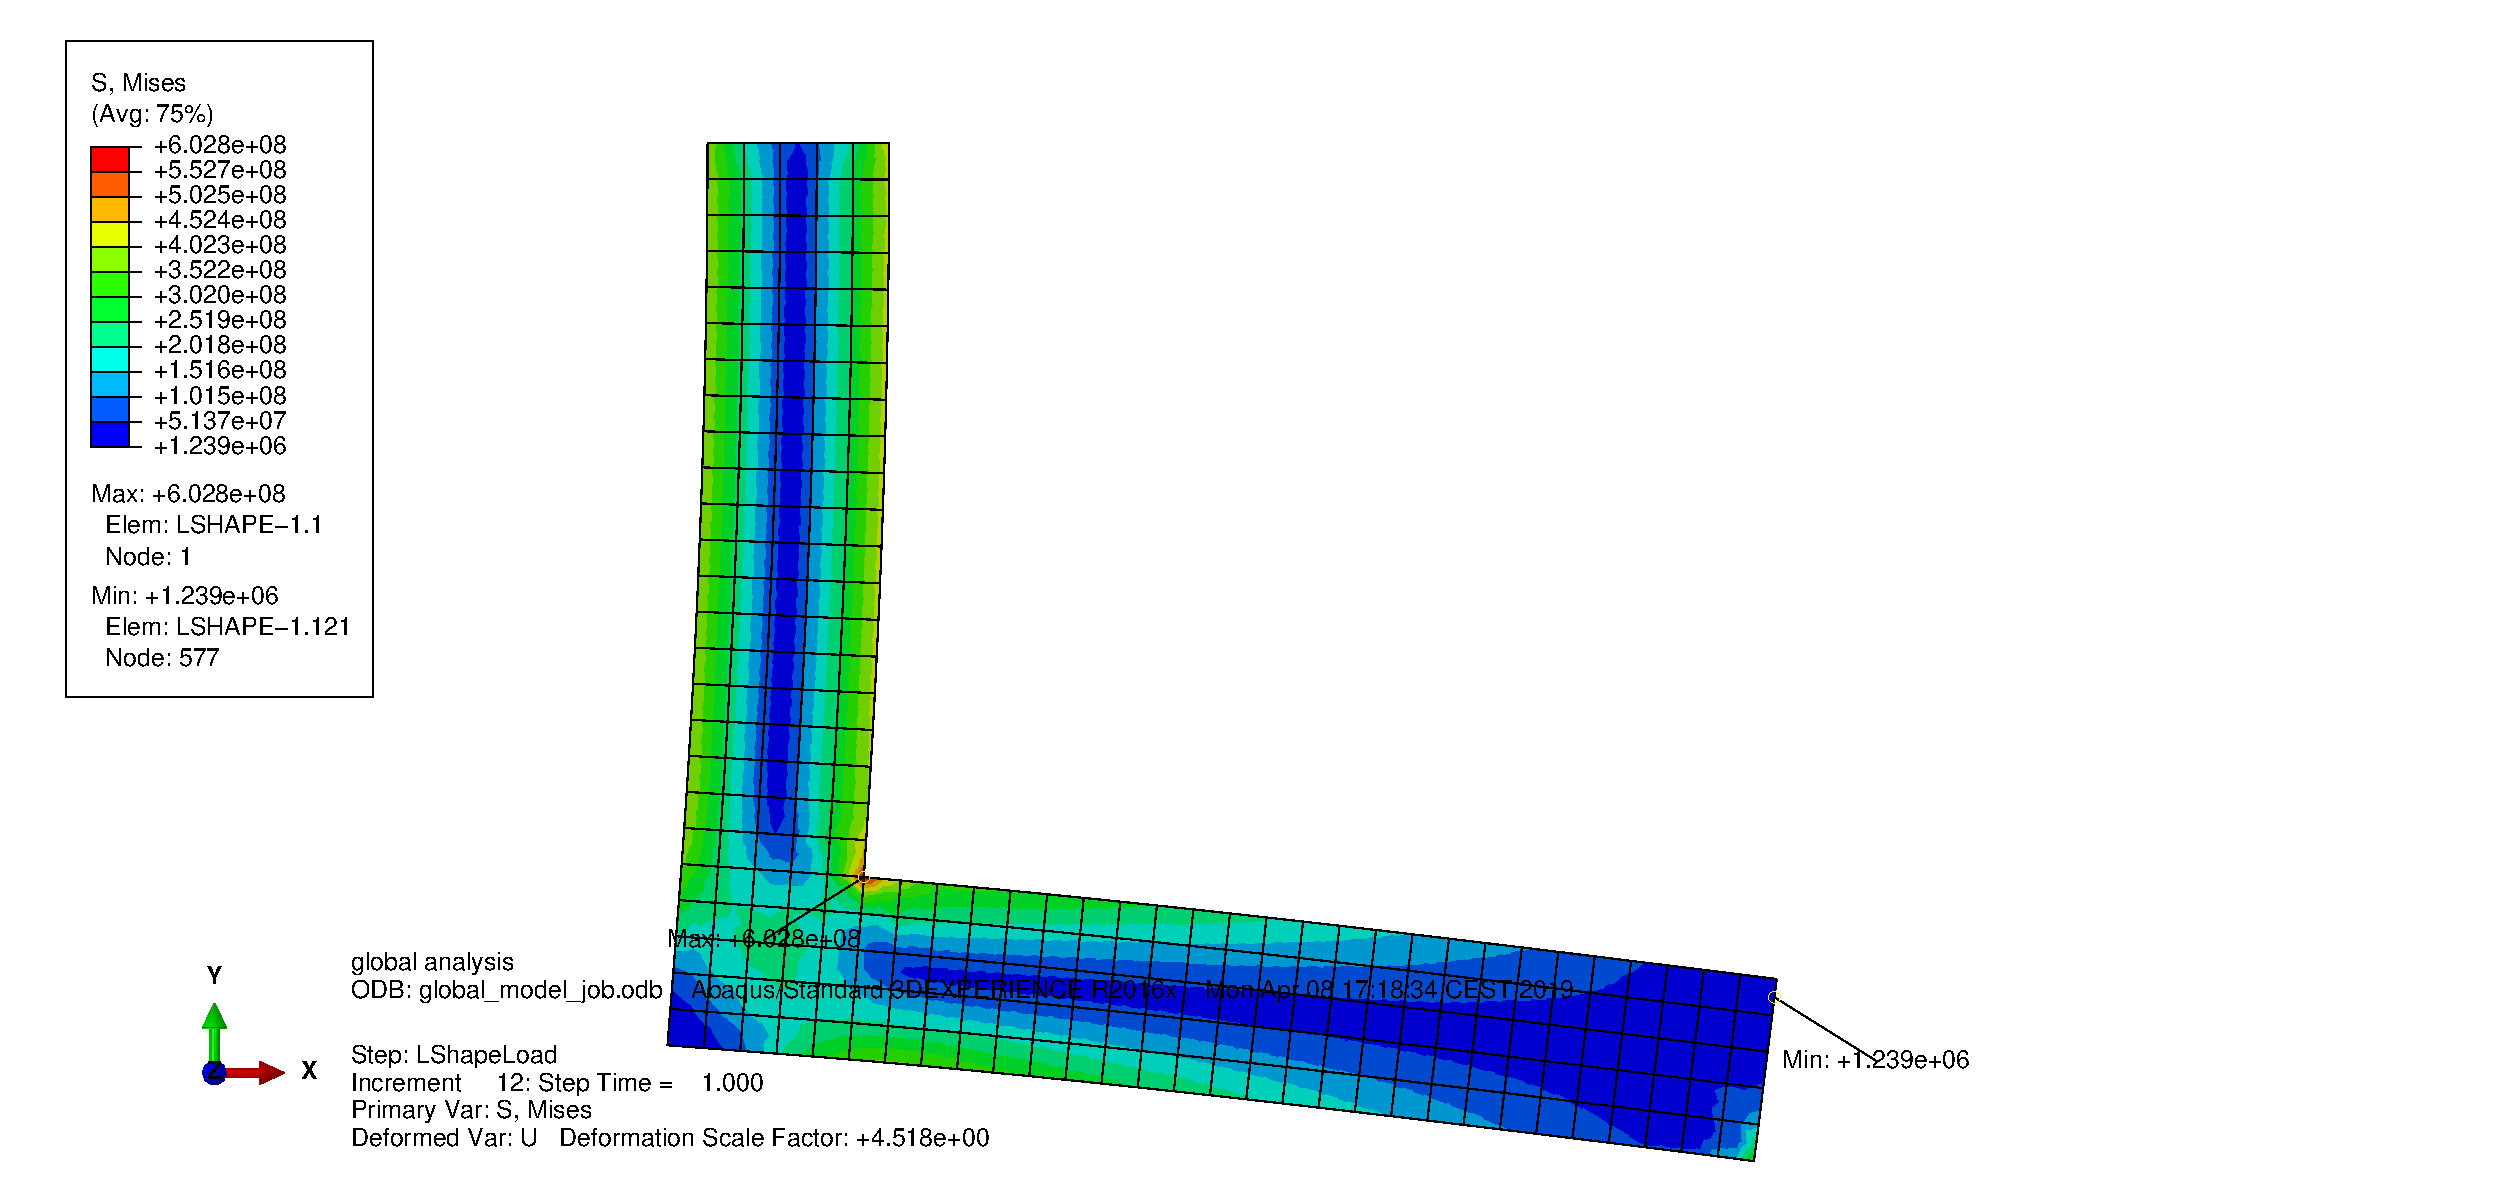
\includegraphics[width=0.95\linewidth]{pics/CPS8R_NoFillet_Global}
    \caption{maximal stress: 603 MPa \\\hspace{\textwidth}minimal stress: 1,24 MPa}
  \end{subfigure}%
  \begin{subfigure}{.5\textwidth}
    \centering
    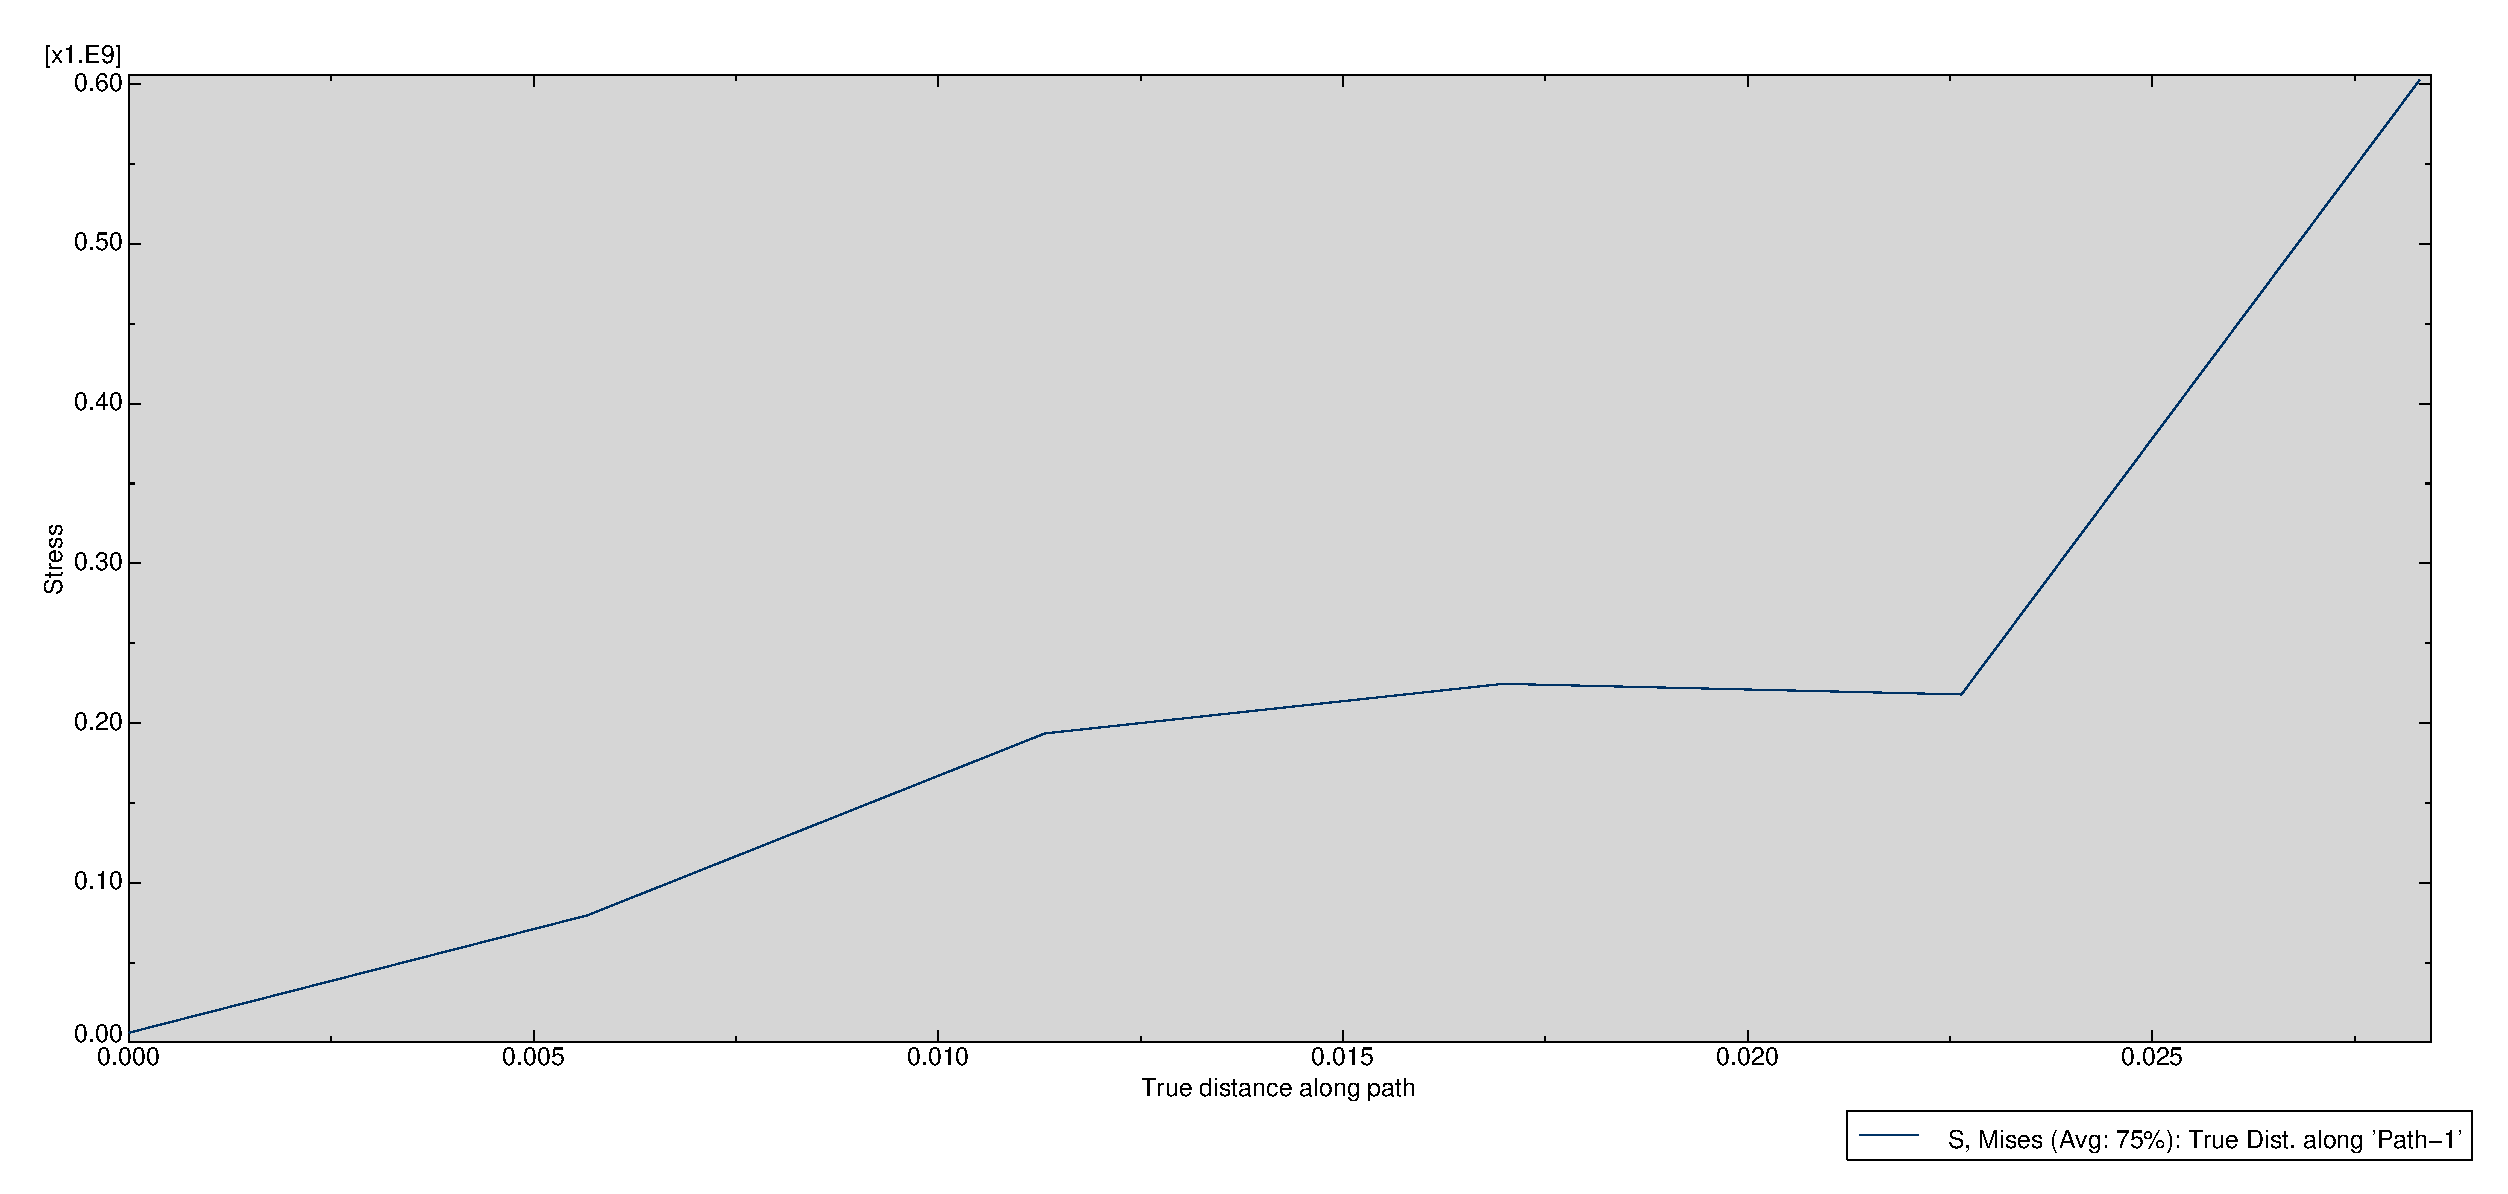
\includegraphics[width=0.95\linewidth]{pics/CPS8R_NoFillet_Global_Plot}
    \caption{Stress (Mises) in N/m$^{2}$ max. 603 N/m$^{2}$}
   \end{subfigure}
  \caption{Global model with no fillet}
\end{figure}

We observe, that the maximum stress value for this setup exceeds the yield stress of 500 MPa. 
We, therefore, expect the beam to be plastically deformed in the region of the inner corner.

\begin{figure}[!htb]
  \centering
  \begin{subfigure}{.5\textwidth}
    \centering
    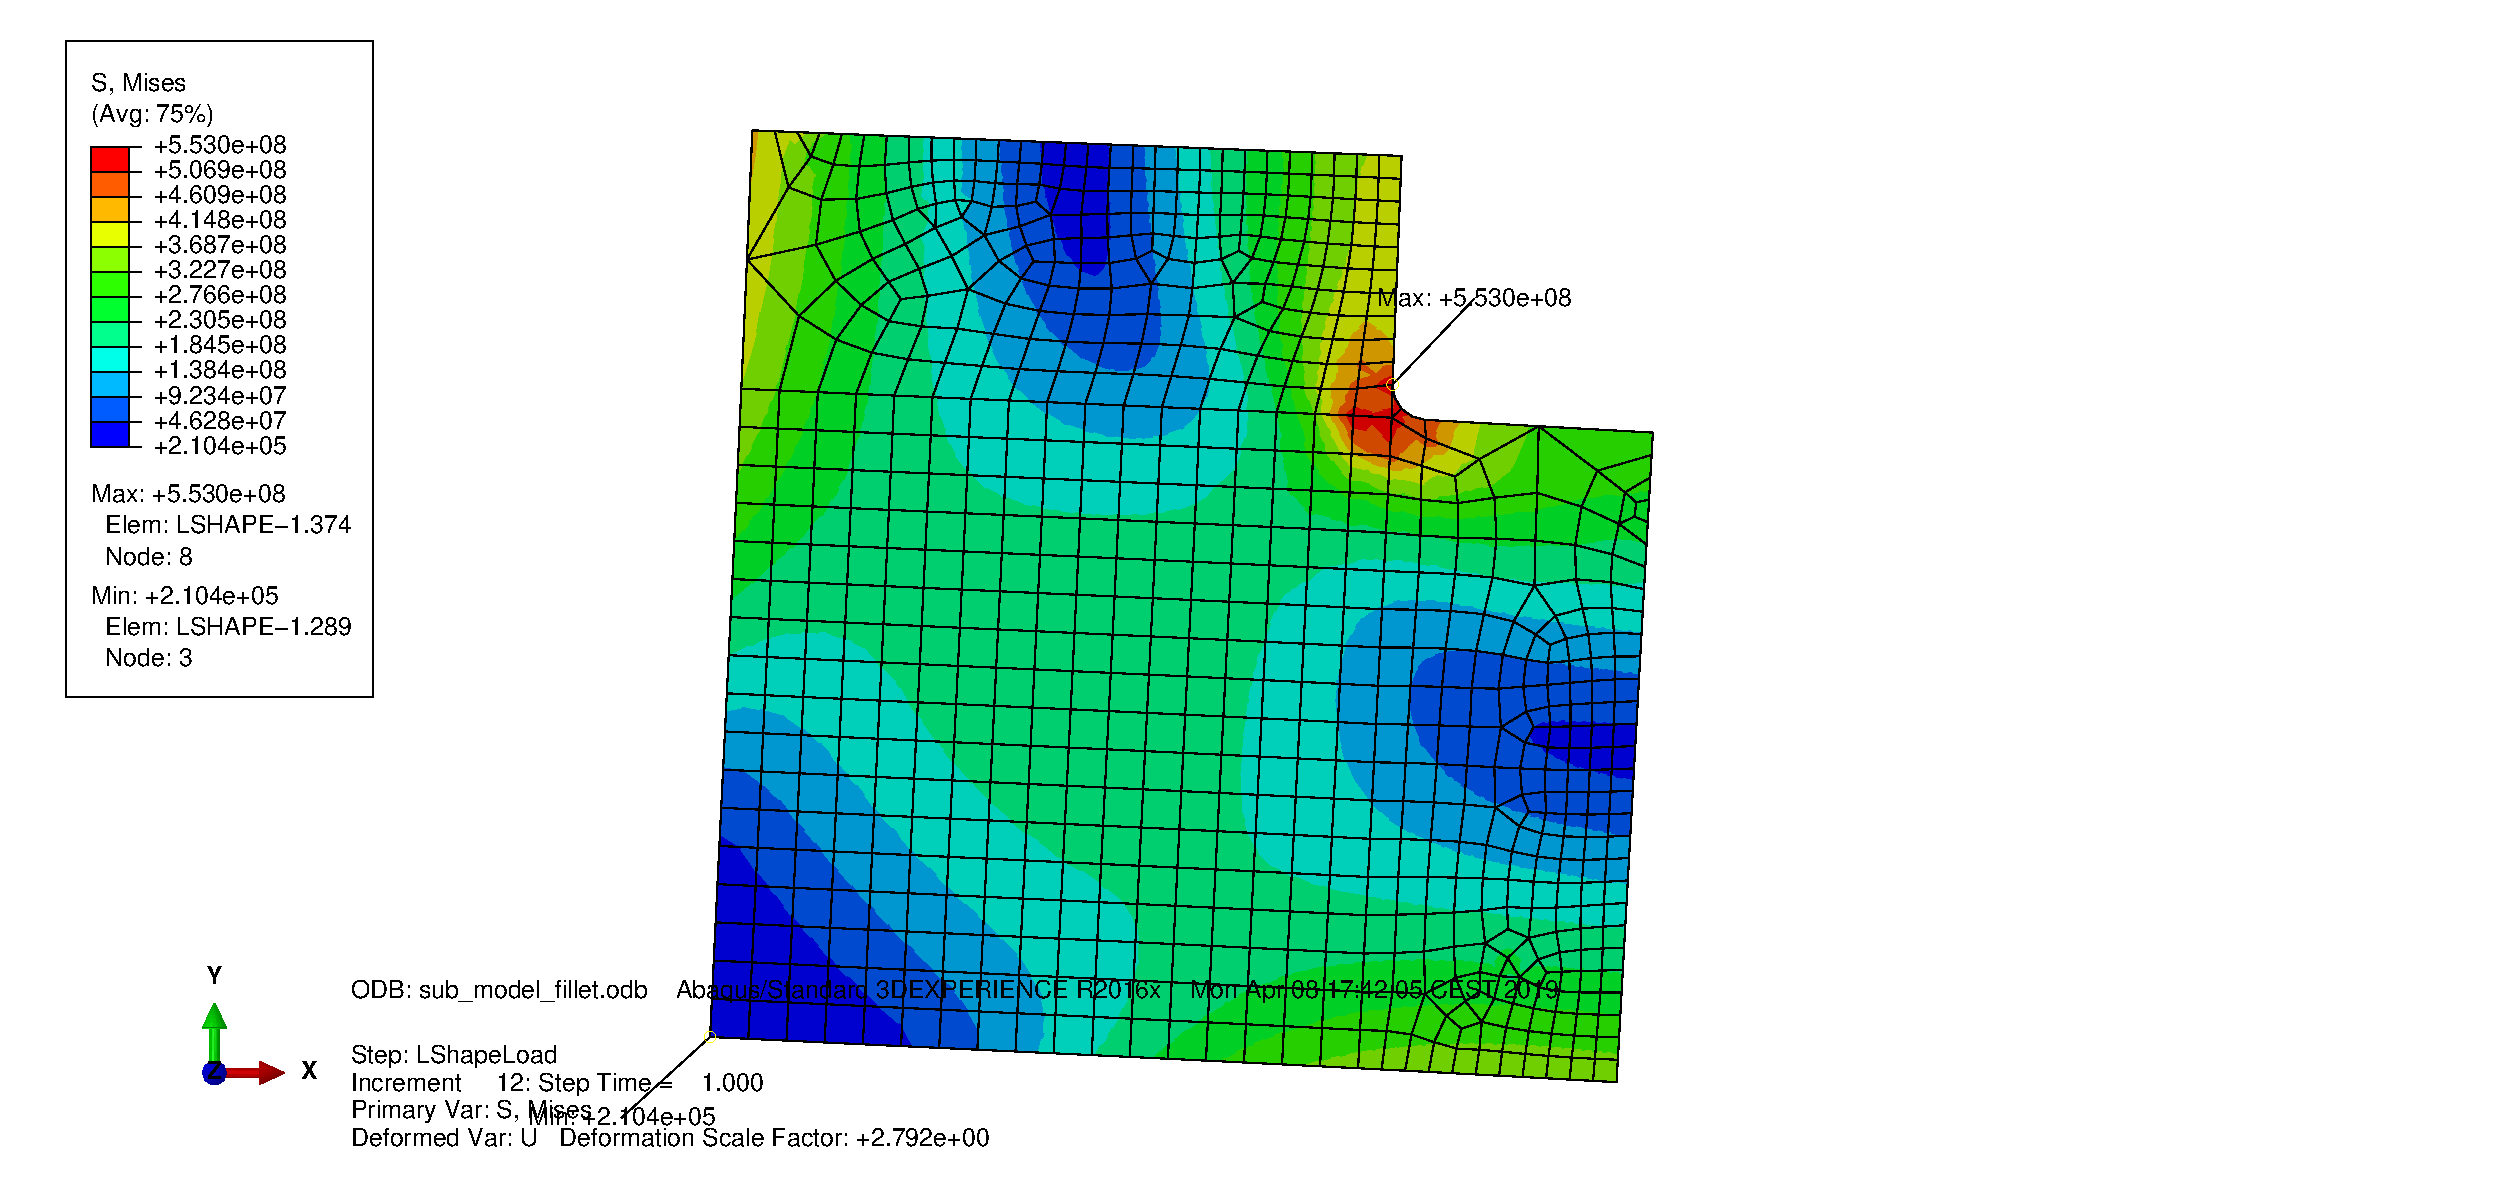
\includegraphics[width=0.95\linewidth]{pics/CPS8R_Fillet}
    \caption{maximal stress: 553 MPa \\\hspace{\textwidth}minimal stress: 0.21 MPa}
  \end{subfigure}%
  \begin{subfigure}{.5\textwidth}
    \centering
    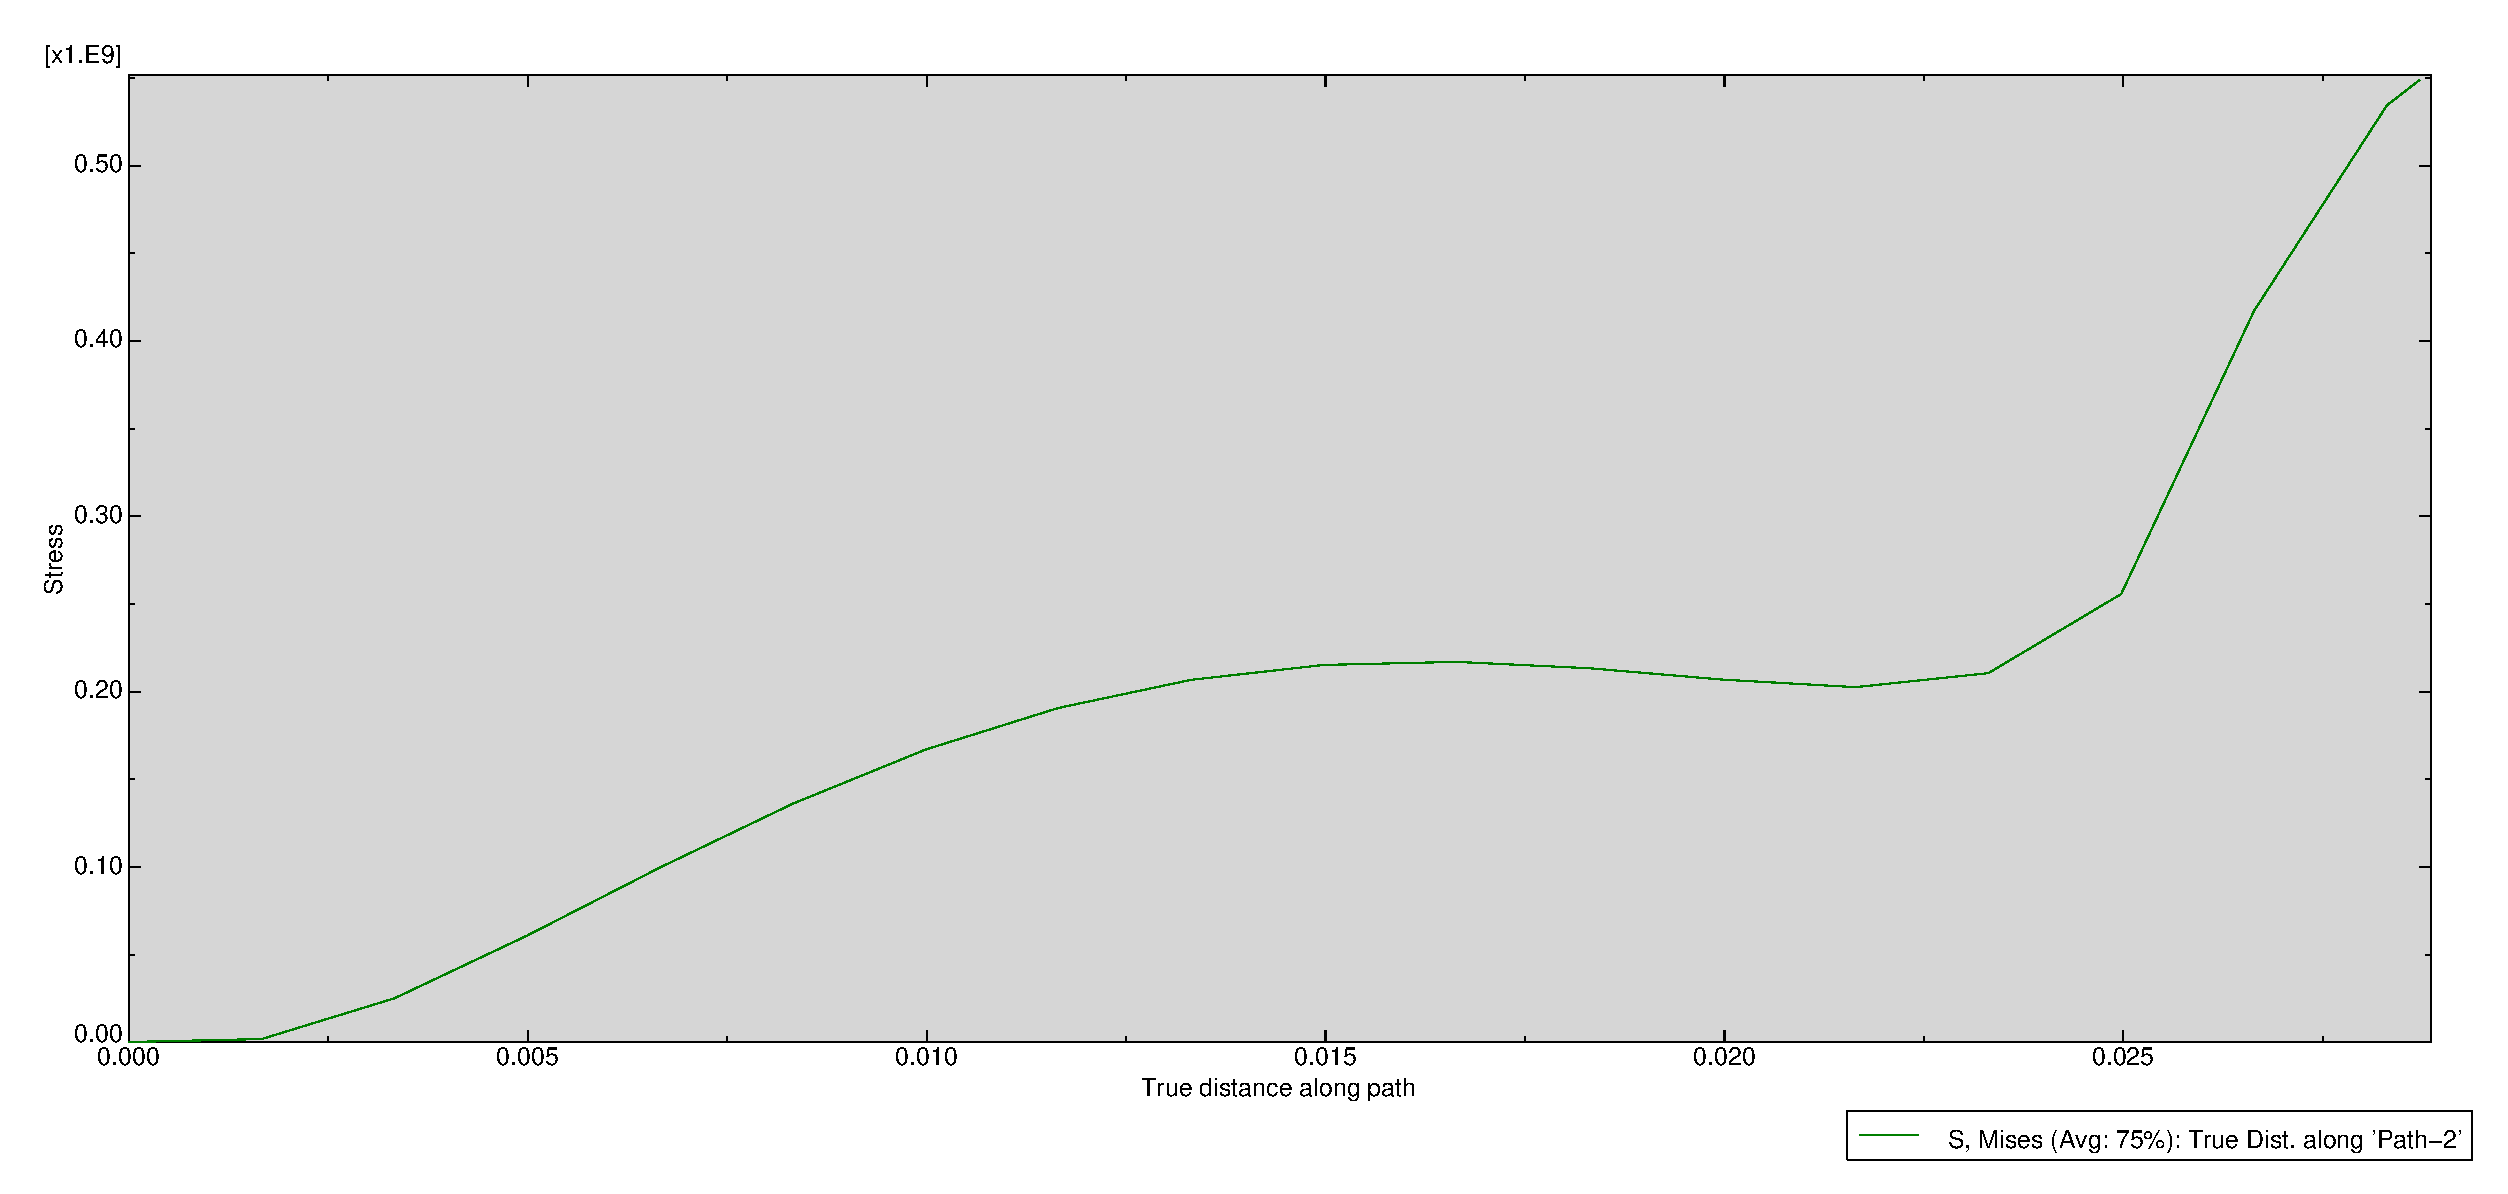
\includegraphics[width=0.95\linewidth]{pics/CPS8R_Fillet_Plot}
    \caption{Stress (Mises) in N/m$^{2}$ max. 553 N/m$^{2}$}
   \end{subfigure}
  \caption{Submodel with 1mm fillet}
\end{figure}

In the submodel with the 1mm fillet, we observe an evenly distributed stress pattern. Also,
the maximum value for stress has decreased by about 50 MPa. From a mechanical point of view, 
the round corner offers a smoother distribution of internal stresses because the lines of 
forces in a material are not interrupted. However, the maximum stress is still the yield 
stress of our material, we still expect it to deform.
\pagebreak

\begin{figure}[!htb]
  \centering
  \begin{subfigure}{.5\textwidth}
    \centering
    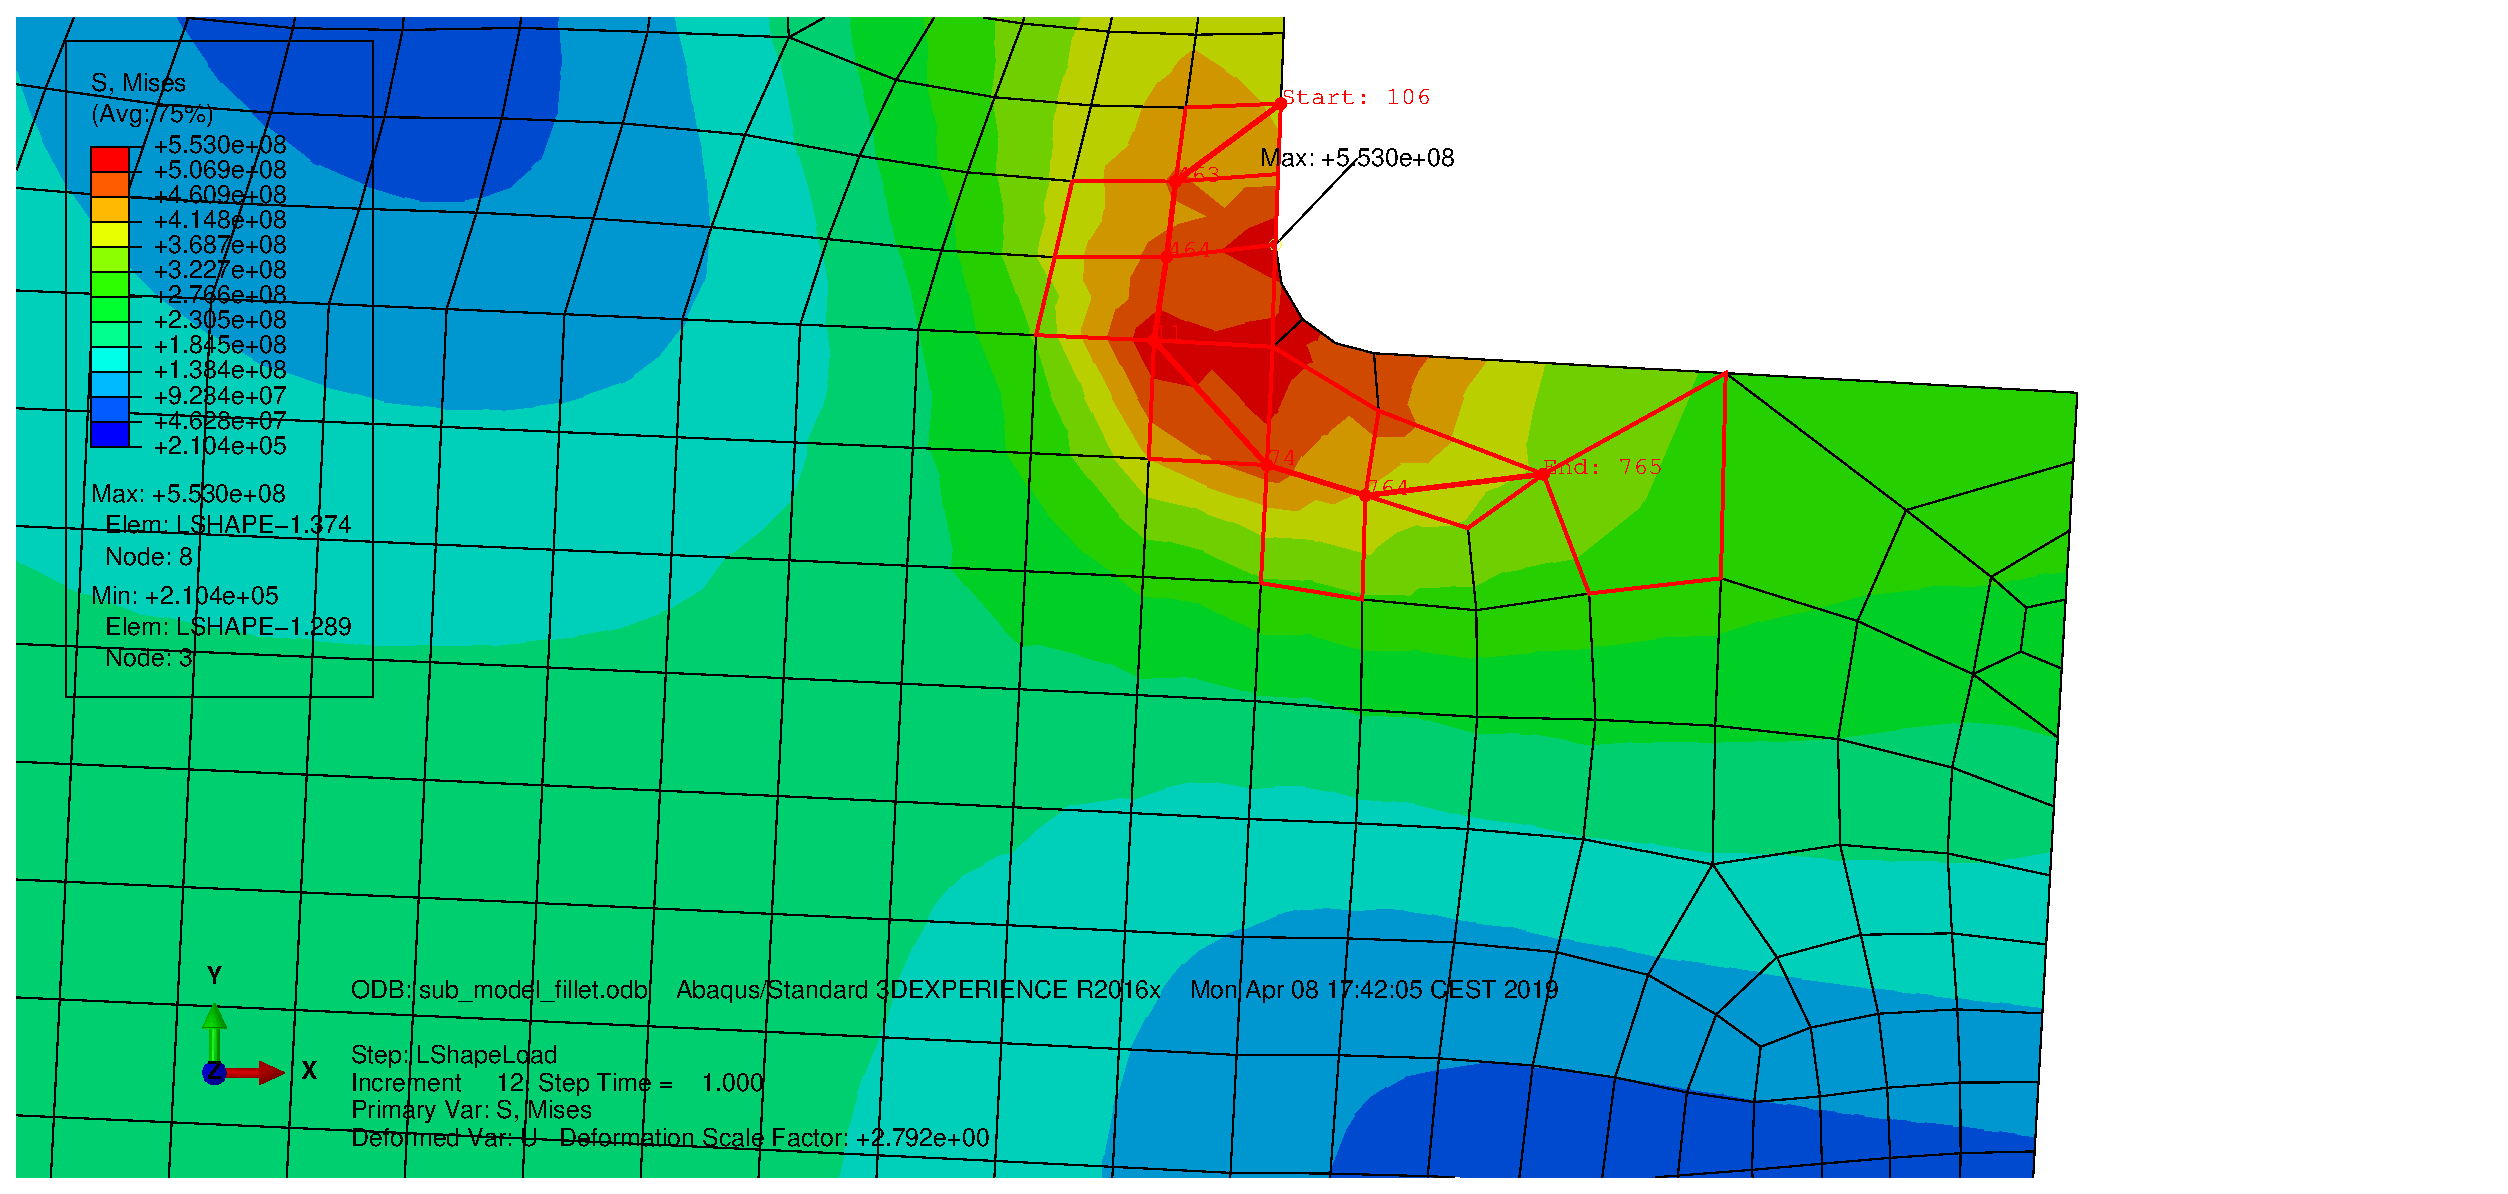
\includegraphics[width=0.95\linewidth]{pics/CPS8R_Fillet_Plot_Circle}
    \caption{Path around the inner corner}
  \end{subfigure}%
  \begin{subfigure}{.5\textwidth}
    \centering
    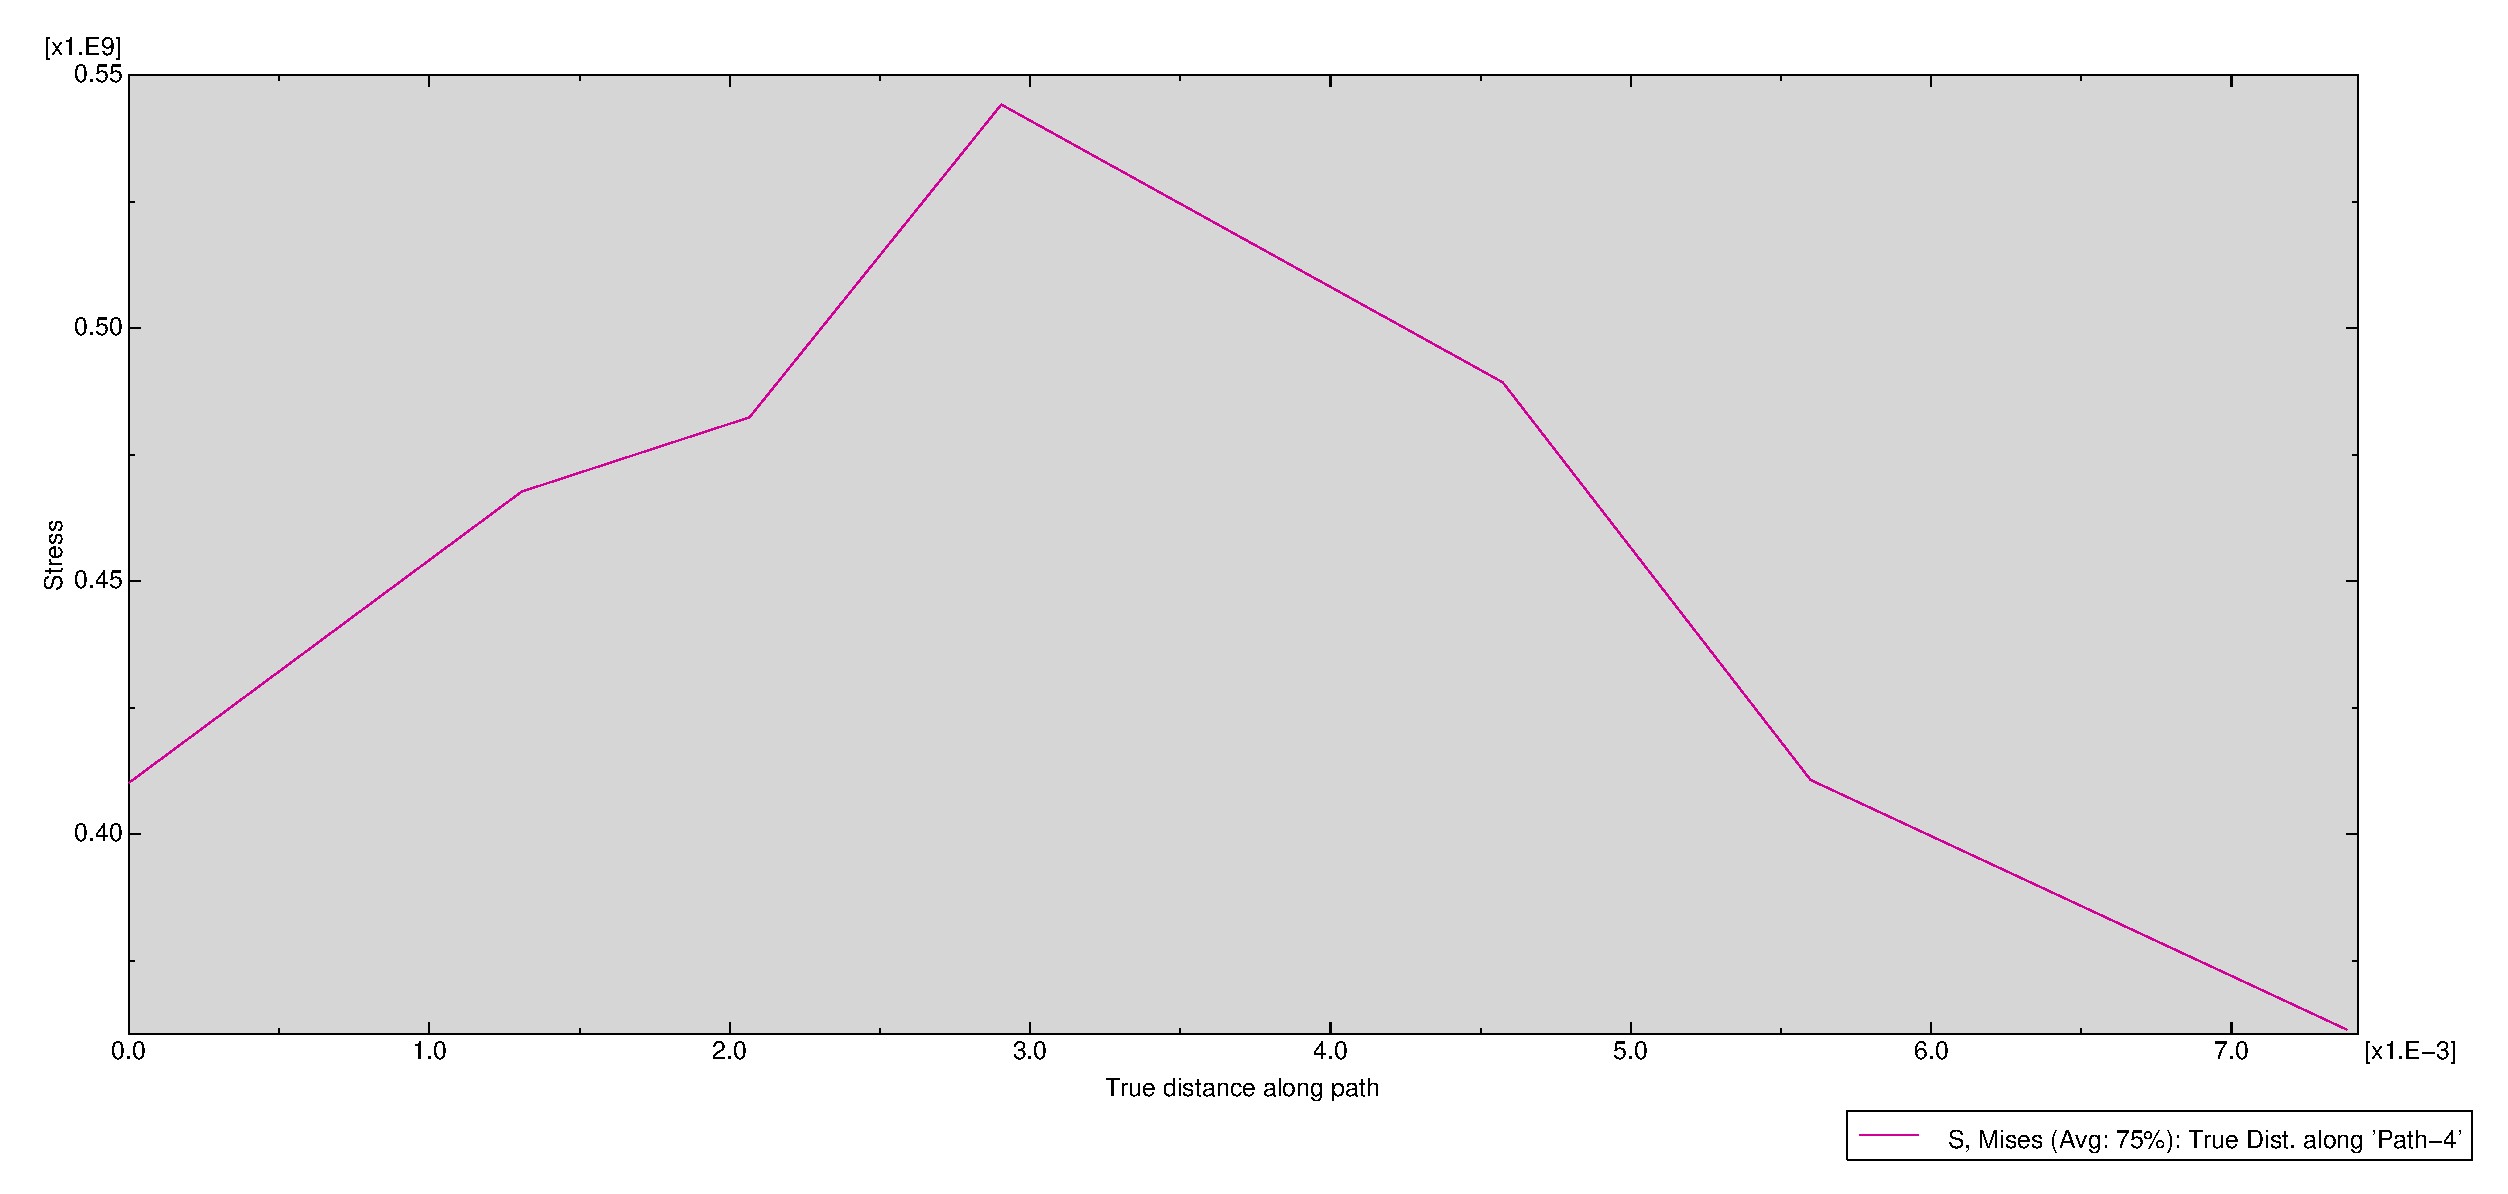
\includegraphics[width=0.95\linewidth]{pics/CPS8R_Fillet_Plot_Circle_Plot}
    \caption{Stress (Mises) in N/m$^{2}$ around the inner corner max. approx. 550 N/m$^{2}$}
   \end{subfigure}
  \caption{Submodel with 1mm fillet}
\end{figure}

We observe that the stresses are highest in the apex of the corner and decrease rapidly with 
distance. The max stress of 553 Mpa is not reached in this plot because it represents only one force line.

\begin{figure}[!htb]
  \centering
  \begin{subfigure}{.5\textwidth}
    \centering
    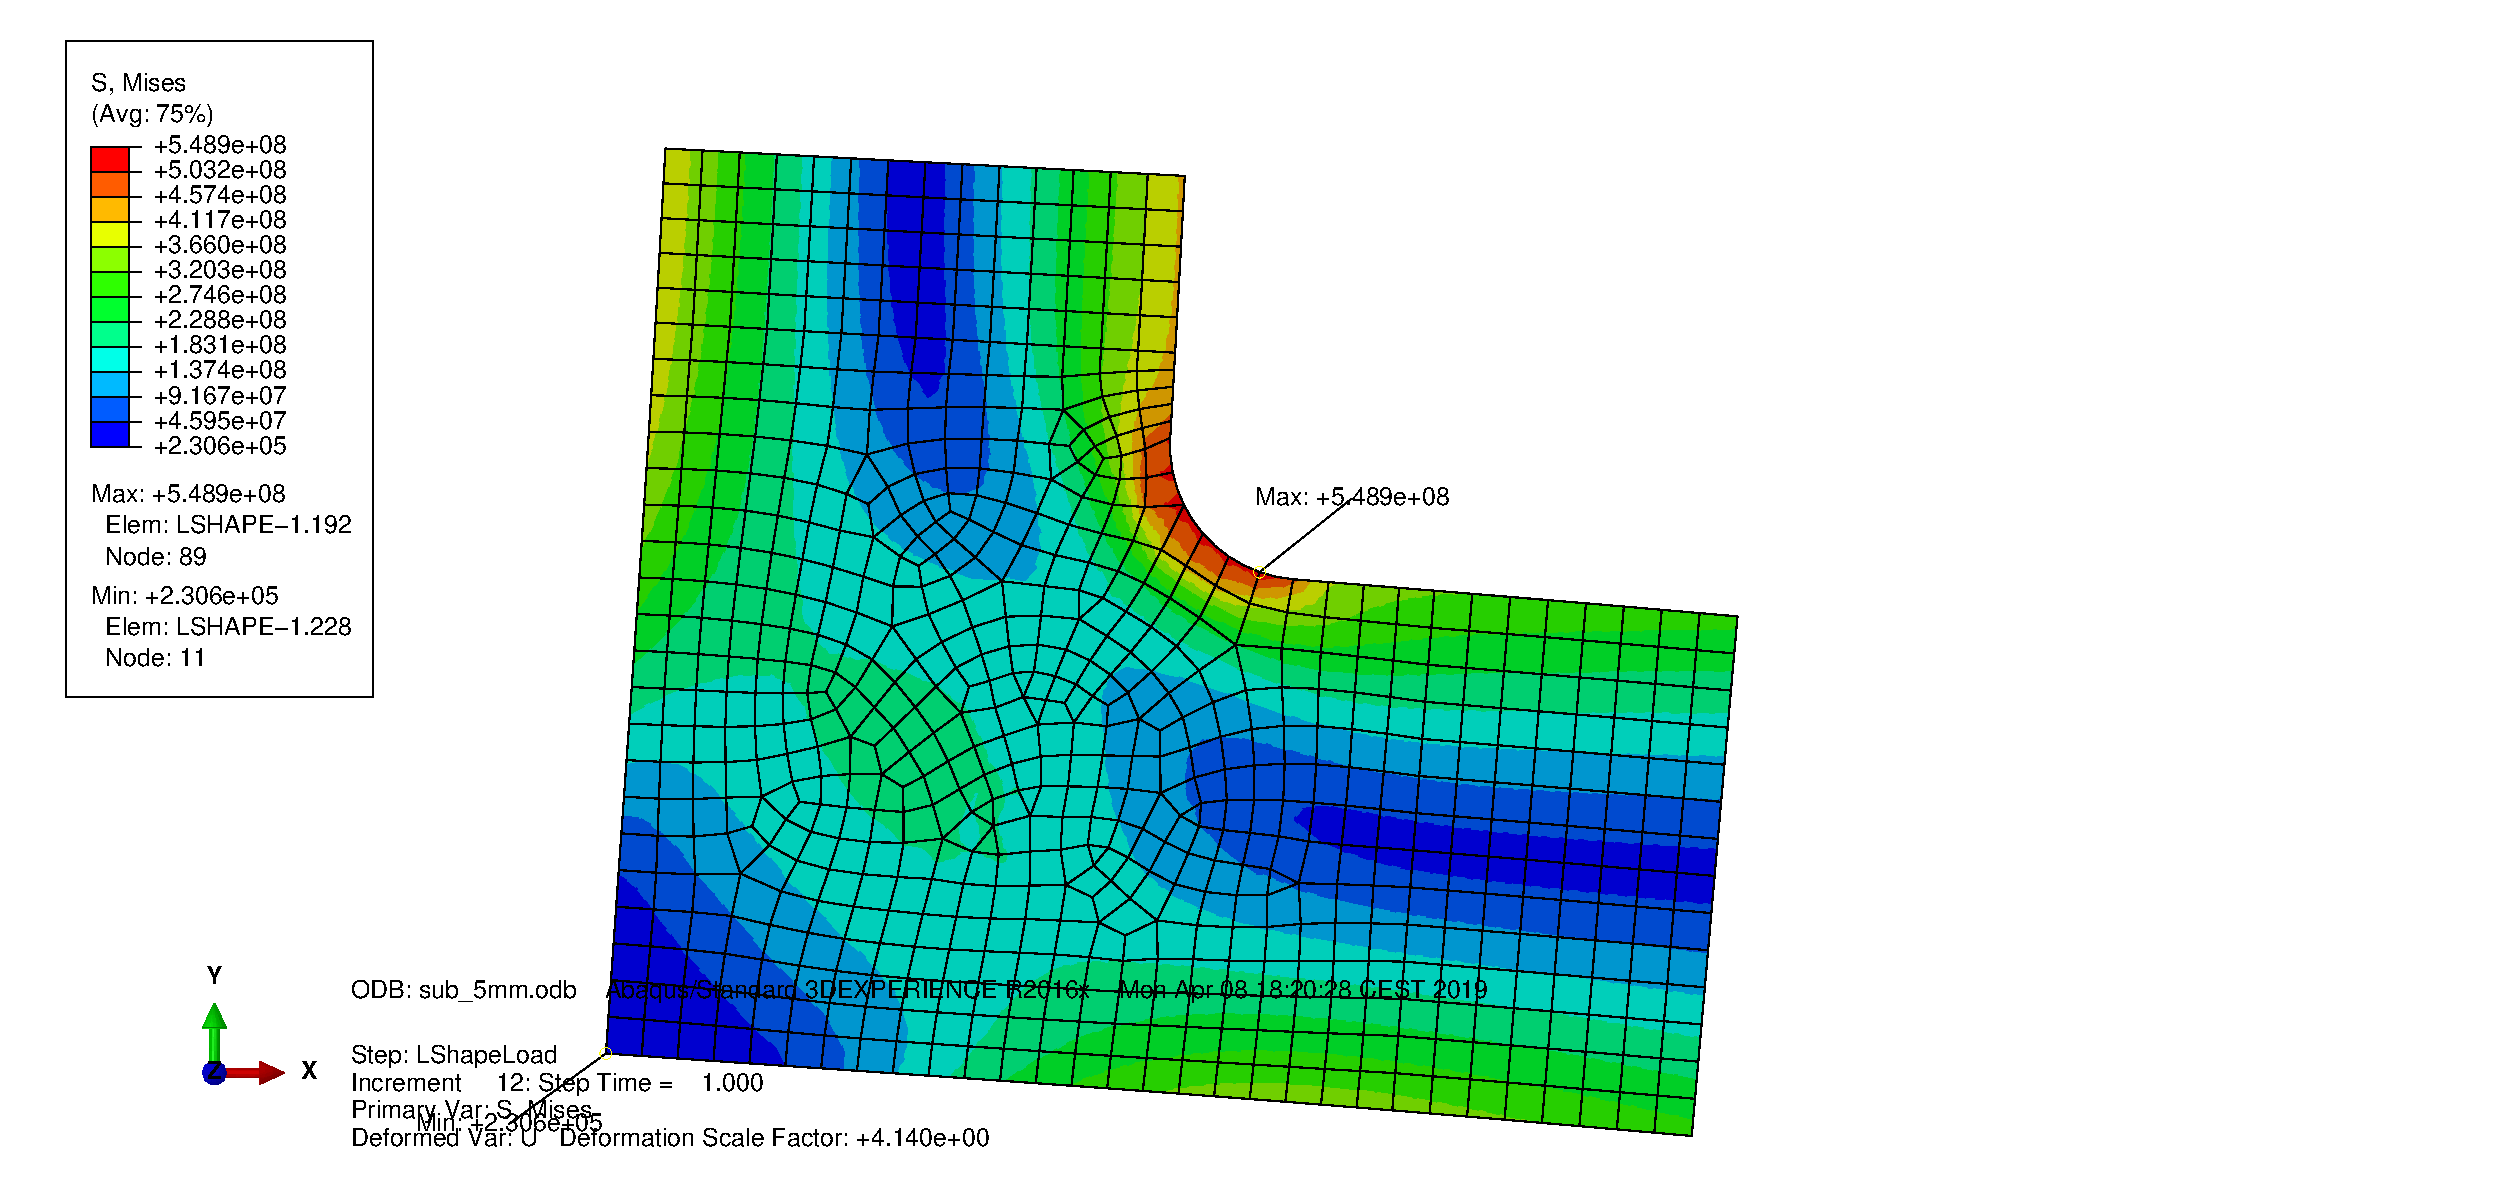
\includegraphics[width=0.95\linewidth]{pics/CPS8R_Fillet_Plot_Circle_Plot_5mm}
    \caption{maximal stress: 549 MPa \\\hspace{\textwidth}minimal stress: 0.23 MPa}
  \end{subfigure}%
  \begin{subfigure}{.5\textwidth}
    \centering
    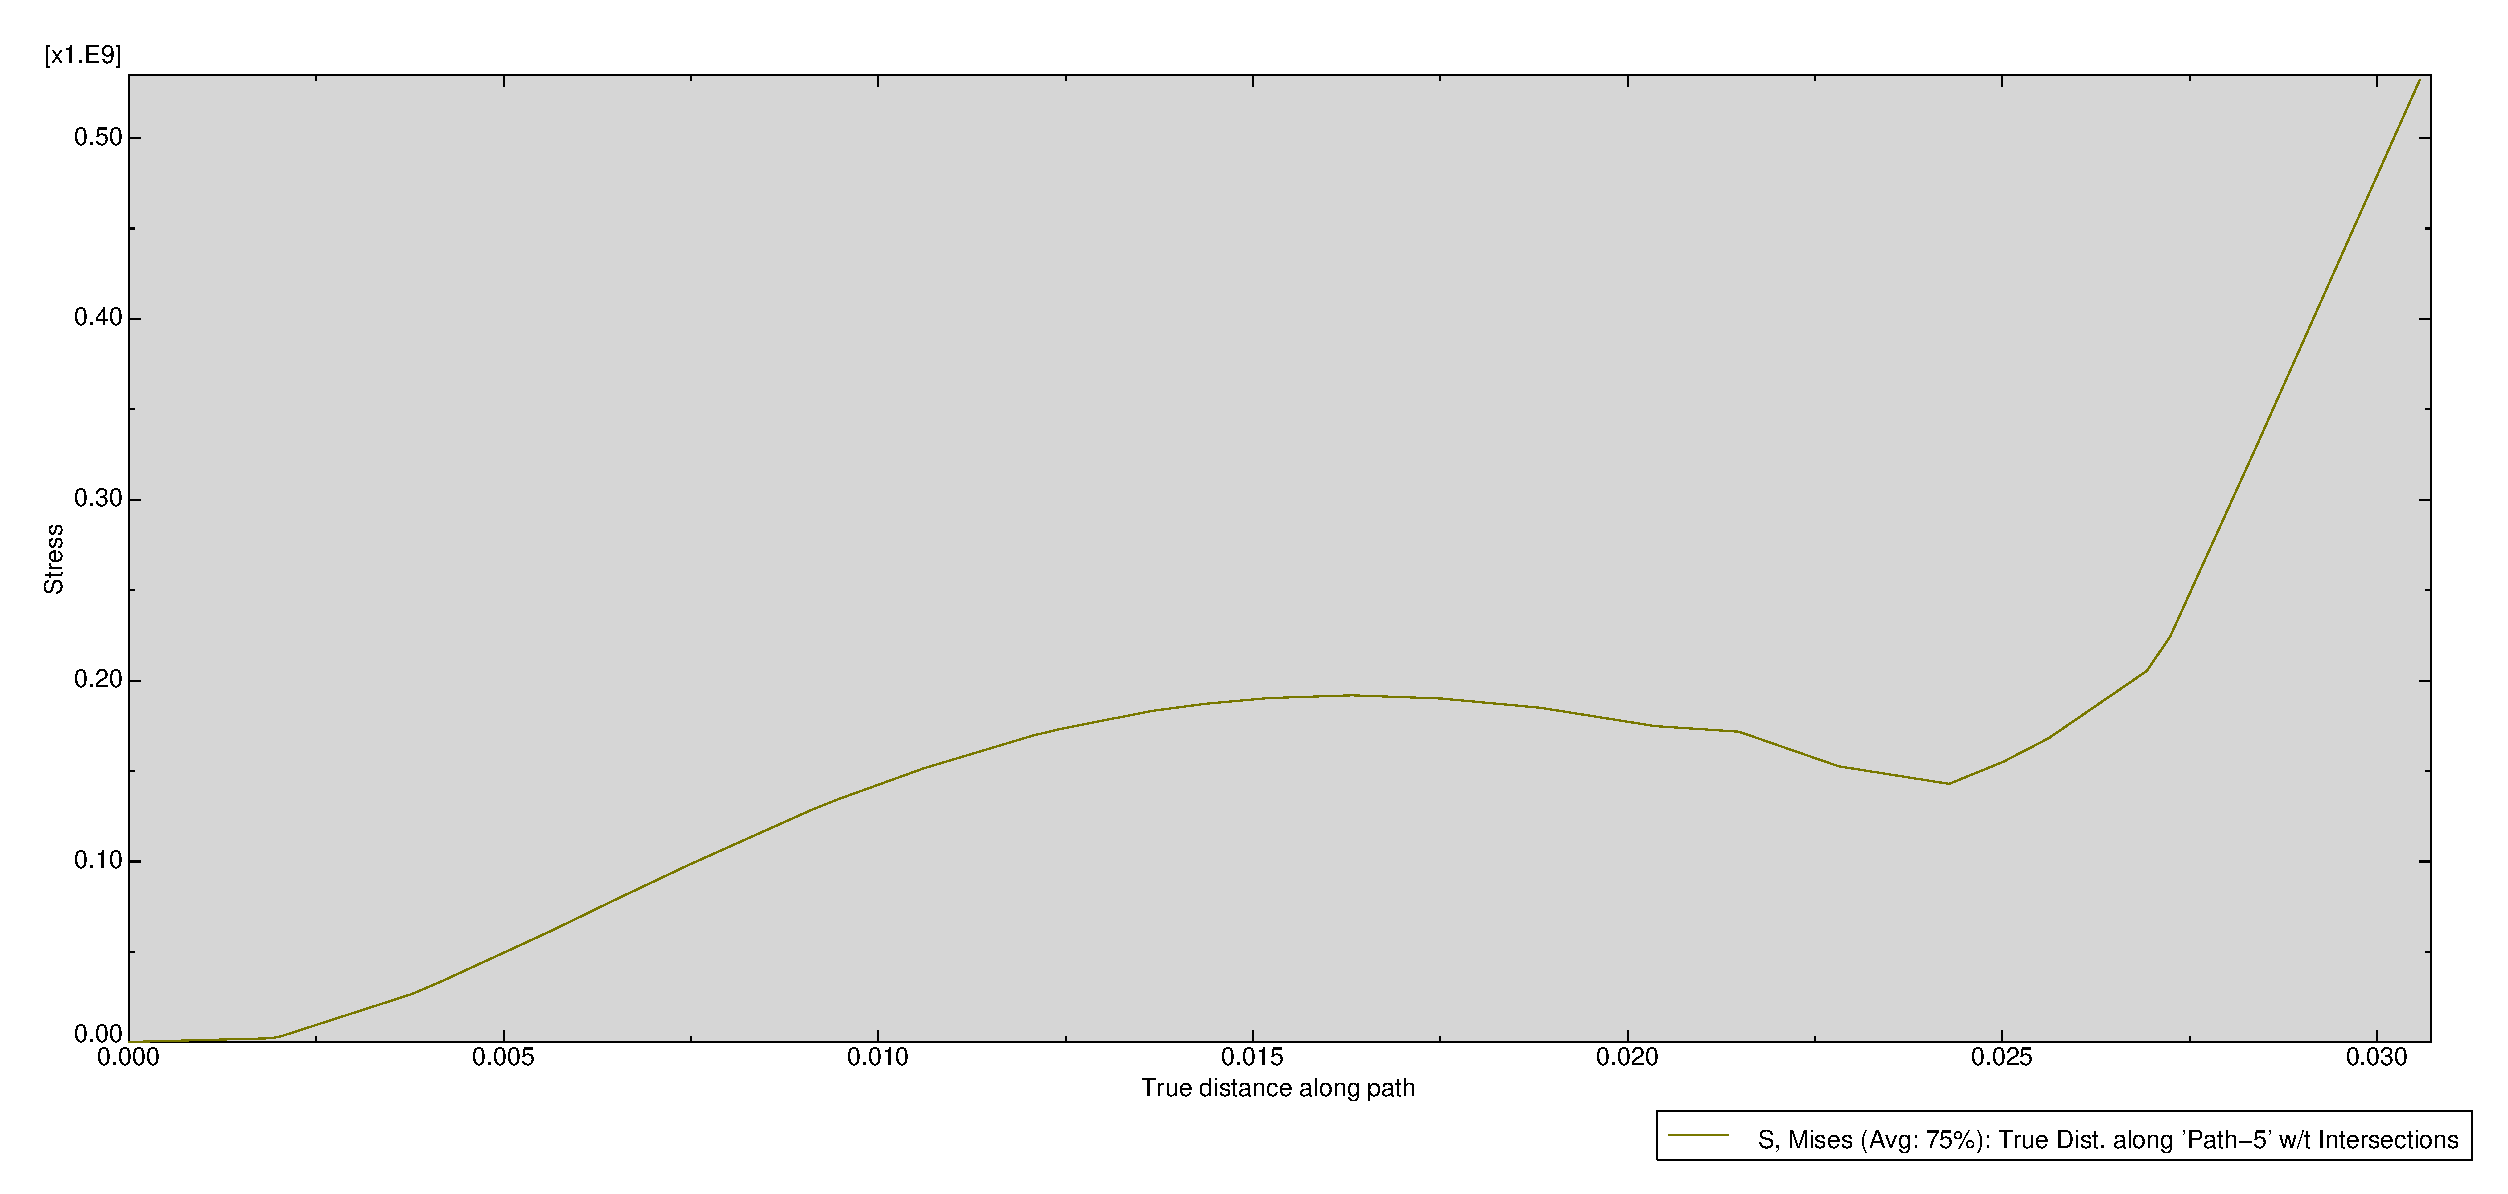
\includegraphics[width=0.95\linewidth]{pics/CPS8R_Fillet_Plot_Circle_Plot_5mm_plot}
    \caption{Stress (Mises) in N/m$^{2}$ around the inner corner max. approx. 500 N/m$^{2}$}
   \end{subfigure}
  \caption{Submodel with 5mm fillet}
\end{figure}

The 5mm fillet causes a minor decrease in maximum stress value. However, the region 
of high stresses is elongated and doesn't reach as deep into the beam compared to the smaller fillet.
\subsection{Conclusion}
The introduction of a fillet in a sharp corner offers a significant decrease in maximum stresses. Even a 
small fillet as a big impact on the model, respectively on the result output. Even though the yield stress 
of the material is still below the maximum stresses (in this exercise), we recognize the notable impact to 
be crucial for any construction project. In order to achieve a suitable mesh around big fillets, a 
repartitioning of the model can be necessary. 


% hahahfootnote \footnote{guguseli}

\pagebreak
\begin{thebibliography}{9}
  \bibitem{latexcompanion} 
  Michel Goossens, Frank Mittelbach, and Alexander Samarin. 
  \textit{The \LaTeX\ Companion}. 
  Addison-Wesley, Reading, Massachusetts, 1993.
   
  \bibitem{einstein} 
  Albert Einstein. 
  \textit{Zur Elektrodynamik bewegter K{\"o}rper}. (German) 
  [\textit{On the electrodynamics of moving bodies}]. 
  Annalen der Physik, 322(10):891–921, 1905.
   
  \bibitem{knuthwebsite} 
  Knuth: Computers and Typesetting,
  \\\texttt{http://www-cs-faculty.stanford.edu/\~{}uno/abcde.html}
\end{thebibliography}


\end{document}